\documentclass[14pt]{article}
 
\usepackage[margin=1in]{geometry} 
% \documentclass[UTF8]{ctexart}
\usepackage{fancyhdr}
\usepackage{extramarks}
\usepackage{amsmath}
\usepackage{amsthm}
\usepackage{amssymb}
\usepackage{ctex}
\usepackage{amsfonts}
\usepackage{mathrsfs}
\usepackage{tikz}
\usepackage[plain]{algorithm}
\usepackage{algpseudocode}
\usepackage{pgfplots}
\usepackage{graphicx}
\usepackage{subfigure}
\usepackage{indentfirst}
\usepackage[numbers]{natbib}
\usepackage{multicol}


\usepackage{listings}
\usepackage{url}
\usepackage[colorlinks,linkcolor=black]{hyperref}
\usetikzlibrary{automata,positioning}
\usetikzlibrary{shapes,arrows}
\usetikzlibrary{positioning}
% \newCJKfontfamily\gothic{IPAexGothic}
% \newCJKfontfamily\mincho{IPAexMincho}
% \numberwithin{equation}{section.subsection}

\topmargin=-0.45in
\evensidemargin=0in
\oddsidemargin=0in
\textwidth=6.5in
\textheight=9.0in
\headsep=0.25in

\linespread{1.1}

\pagestyle{fancy}
\lhead{\hmwkAuthorName}
\chead{\textbf{\hmwkClass}}
\rhead{\hmwkClassInstructor}
\lfoot{\lastxmark}
\cfoot{\thepage}

\renewcommand\headrulewidth{0.4pt}
\renewcommand\footrulewidth{0.4pt}



\newcommand{\n}{\mathbb{N}}
\newcommand{\z}{\mathbb{Z}}
\newcommand{\q}{\mathbb{Q}}
\newcommand{\cx}{\mathbb{C}}
\newcommand{\real}{\mathbb{R}}
\newcommand{\field}{\mathbb{F}}
\newcommand{\ita}[1]{\textit{#1}}
\newcommand{\com}[2]{#1\backslash#2}
\newcommand{\oneton}{\{1,2,3,...,n\}}
\newcommand\idea[1]{\begin{gather*}#1\end{gather*}}
\newcommand\eali[1]{\begin{align*}#1\end{align*}}
\newcommand\ef{\ita{f} }
\newcommand\eff{\ita{f}}
\newcommand\proofs[1]{\begin{proof}#1\end{proof}}
\newcommand\inv[1]{#1^{-1}}
\newcommand\setb[1]{\{#1\}}
\newcommand\en{\ita{n }}
\newcommand{\vbrack}[1]{\langle #1\rangle}
% \newcommand{\r}{\mathrm{r}}

\newcommand{\derivt}[1]{\frac{\mathrm{d}}{\mathrm{d}t} (#1)}
\newcommand{\Derivt}[1]{\frac{\mathrm{D}}{\mathrm{D}t} (#1)}
\newcommand{\derivo}[2]{\frac{\mathrm{d} #1 }{\mathrm{d} #2}}
\newcommand{\Derivo}[2]{\frac{\mathrm{D} #1 }{\mathrm{D} #2}}
\newcommand{\derivoo}[2]{\frac{\mathrm{d}^{2} #1 }{\mathrm{d} #2^{2}}}
\newcommand{\Derivoo}[2]{\frac{\mathrm{D}^{2} #1 }{\mathrm{D} #2^{2}}}
\newcommand{\derivp}[2]{\frac{\partial #1}{\partial #2}}
\newcommand{\derivpp}[2]{\frac{\partial^{2} #1}{\partial #2^{2}}}

\newcommand{\vbe}[1]{\vec{\boldsymbol{e}}_{#1}}
\newcommand{\vbed}[1]{\Dot{\vec{\boldsymbol{e}}}_{#1}}
\newcommand{\csg}[2]{\Gamma^{#1}_{#2}}
\newcommand{\csgd}[3]{\Gamma^{#1}_{#2,#3}}
\newcommand{\g}{\mathrm{g}}
\newcommand{\csge}[3]{\frac{1}{2} \mathrm{g}^{#1\gamma}(\mathrm{g}_{#2\gamma, #3}+\mathrm{g}_{#3 \gamma,#2}-\mathrm{g}_{#2 #3,\gamma})}

\newcommand{\Ricci}[2]{\csgd{\sigma}{#1#2}{\sigma} - \csgd{\sigma}{#1\sigma}{#2} +\csg{\sigma}{\rho \sigma}\csg{\rho}{#1 #2} -\csg{\sigma}{\rho #2}\csg{\rho}{#1\sigma}}




\newenvironment{theorem}[2][Theorem]{\begin{trivlist}\item[\hskip \labelsep {\bfseries #1}\hskip \labelsep {\bfseries #2.}]}{\end{trivlist}}

\newenvironment{lemma}[2][Lemma]{\begin{trivlist}
\item[\hskip \labelsep {\bfseries #1}\hskip \labelsep {\bfseries #2.}]}{\end{trivlist}}
\newenvironment{exercise}[2][Exercise]{\begin{trivlist}
\item[\hskip \labelsep {\bfseries #1}\hskip \labelsep {\bfseries #2.}]}{\end{trivlist}}
\newenvironment{reflection}[2][Reflection]{\begin{trivlist}
\item[\hskip \labelsep {\bfseries #1}\hskip \labelsep {\bfseries #2.}]}{\end{trivlist}}
\newenvironment{proposition}[2][Proposition]{\begin{trivlist}
\item[\hskip \labelsep {\bfseries #1}\hskip \labelsep {\bfseries #2.}]}{\end{trivlist}}
\newenvironment{corollary}[2][Corollary]{\begin{trivlist}
\item[\hskip \labelsep {\bfseries #1}\hskip \labelsep {\bfseries #2.}]}{\end{trivlist}}
%  \hypersetup{
%  colorlinks,
%  linkcolor=blue
%  }


% \newcommand{\hmwkTitle}{000}
% \newcommand{\hmwkDueDate}{2020年9月20日}
\newcommand{\hmwkClass}{Dark Energy Theorem and Observation}
% \newcommand{\hmwkClassTime}{}
\newcommand{\hmwkClassInstructor}{Wang Zhengyi}
\newcommand{\hmwkAuthorNameCover}{Wang Zhengyi 201711160128}
\newcommand{\hmwkAuthorName}{BNU-DOA}



%
% Title Page
%

\title{
    \begin{center}
      
\includegraphics[scale=1.6]{BNU_name.jpg}
    \end{center}
    \vspace{2.5in}
    \Huge{\textbf{\hmwkClass}}\\
    % \vspace{0.1in} \large{\textbf{\hmwkDueDate}} \\
    \vspace{1in}
}
\author{\textbf{\hmwkAuthorNameCover}}
\date{}
\begin{document}
\maketitle
\pagebreak

\section{Dark Energy Theorem}

\subsection{FRLW Metric}
\quad\\
\textbf{For a 3-D hyper-sphere,the distance between two points of space is:}
\[
ds^{2} = f(r)dr^{2}+r^{2}d\theta +r^{2}\sin^{2}\theta\tag{1.1.1}
\]
\textbf{Gaussian Curvature:}
\[
k=\frac{1}{2f^{2}(r)r}\derivo{f(r)}{r}\tag{1.1.2}
\]
\textbf{Solution:}
\[
f(r)=\frac{1}{C-kr^{2}} \tag{1.1.3}
\]
\textbf{Let C=1,and introduce cosmological scale :}
\[
K=-\frac{k}{a^{2}} \tag{1.1.4}
\]
\[
-c^{2}d\tau^{2} = -c^{2}dt^{2}+a^{2}[\displaystyle\frac{dr^{2}}{1-Kr^{2}}+r^{2}(d\theta^{2}+\sin^{2}\theta d\phi^{2})] \tag{1.1.5}
\]
\begin{align*}
\g_{\mu\nu}=
\left[
    \begin{array}{cccc}
        -c^{2} & 0 & 0 & 0\\\\
        0 & \frac{a^{2}}{1-Kr^{2}} & 0 & 0\\\\
        0 & 0 & a^{2}r^{2} & 0\\\\
        0 & 0 & 0 & a^{2}r^{2}\sin^{2}\theta\\\\
    \end{array}
\right]    \tag{1.1.6}
\end{align*}
\begin{align*}
\g_{00} = -c^{2},\quad \g_{11} = \frac{a^{2}}{1-Kr^{2}},&\quad \g_{22} = a^{2}r^{2},\quad \g_{33}=a^{2}r^{2}\sin^{2}\theta \tag{1.1.7}\\
\g^{00} = -\frac{1}{c^{2}},\quad \g^{11} = \frac{1-Kr^{2}}{a^{2}},&\quad \g^{22} = \frac{1}{a^{2}r^{2}},\quad \g^{33}=\frac{1}{a^{2}r^{2}\sin^{2}\theta} \tag{1.1.8}\\
\g_{00,\gamma} = 0 \quad& (\gamma = 0,1,2,3) \tag{1.1.9}\\
\g_{11,0} = \frac{1}{c^{2}}\frac{2a\dot{a}}{1-Kr^{2}},\quad\g_{11,1} &= \frac{2a^{2}Kr}{(1-Kr^{2})^{2}},\quad\g_{11,2} =\g_{11,3} =0\tag{1.1.10}\\
\g_{22,0} = 2a\dot{a}r^{2},\quad\g_{22,1}&=2a^{2}r,\quad\g_{22,2} =\g_{22,3} =0\tag{1.1.11}\\
\g_{33,0} = 2a\dot{a}r^{2}\sin^{2}\theta,\quad\g_{33,1}=2a^{2}&r\sin^{2}\theta,\quad\g_{33,2}=2a^{2}r\sin^{2},\quad\g_{33,3} =0\tag{1.1.12}\\
\end{align*}

\subsection{Christoffel Symbols}
\quad\\

\[
\csg{\sigma}{\mu\nu}=\csge{\sigma}{\mu}{\nu}\tag{1.2.1}
\]
\textbf{Non-Zero Components of Christoffel Symbols:}
\begin{align*}
\csg{0}{11} &= \csge{0}{1}{1}\\
            &= \quad -\frac{1}{2}\g^{00}\g_{11,0}
            = \frac{1}{c^{2}}\frac{a\Dot{a}}{1-Kr^{2}}\tag{1.2.2}\\
\csg{0}{22} &= \csge{0}{2}{2}\\
            &= -\frac{1}{2}\g^{00}\g_{22,0}
            = \frac{1}{c^{2}}a\Dot{a}r^{2}\tag{1.2.3}\\
\csg{0}{33} &= \csge{0}{3}{3} \\
            &= -\frac{1}{2}\g^{00}\g_{33,0}
            = \frac{1}{c^{2}}a\Dot{a}r^{2}\sin^{2}\theta\tag{1.2.4}\\
\csg{i}{j0} &= \csge{i}{j}{0} \\
            &= \frac{1}{2}\g^{ii}\g_{ij,0}
            = \frac{\Dot{a}}{a}\delta^{i}_{j}\tag{1.2.5}\\
\csg{1}{11} &= \csge{1}{1}{1} \\
            &= \frac{1}{2}\g^{11}\g_{11,1}
            = \frac{Kr}{1-Kr^{2}}\tag{1.2.6}\\
\csg{1}{22} &= \csge{1}{2}{2} \\
            &= -\frac{1}{2}\g^{11}\g_{22,1}
            = -r(1-Kr^{2}) \tag{1.2.7}\\   
\csg{1}{33} &= \csge{1}{3}{3} \\
            &= -\frac{1}{2}\g^{11}\g_{33,1}
            = -r\sin^{2}\theta(1-Kr^{2}) \tag{1.2.8}\\  
\csg{2}{12} &=  \csge{2}{1}{2}\\
            &= \frac{1}{2}\g^{22}\g_{22,1}
            = \frac{1}{r} \tag{1.2.9}\\
\csg{3}{13} &= \csge{3}{1}{3} \\
            &= \frac{1}{2}\g^{33}\g_{33,1}
            = \frac{1}{r}  \tag{1.2.10}\\ 
\csg{3}{23} &= \csge{3}{2}{3} \\
            &= \frac{1}{2}\g^{33}\g_{33,2}
            = -\sin \theta \cos \theta  \tag{1.2.11}\\
\csg{2}{33} &= \csge{2}{3}{3} \\
            &= \frac{1}{2}\g^{22}\g_{33,2}
            = \cot \theta  \tag{1.2.12}
\end{align*}

for\(i,j=1,2,3\)
\subsection{Ricci Tensor}

\[
R_{\mu\nu}  = \Ricci{\mu}{\nu} \tag{1.3.1}
\]
\textbf{Non-Zero Components of Ricci Tensor:}
\begin{align*}
R_{00}  &= \Ricci{0}{0}\\
        &= \csg{0}{00,0} -\csg{\sigma}{0\sigma,0}  +\csg{\sigma}{0\sigma} \csg{0}{00} - \csg{\sigma}{\sigma 0} \csg{\sigma}{0\sigma}\\ 
        &= 0-3\frac{\ddot{a}a-\dot{a}^{2}}{a^{2}}+0-3(\frac{\dot{a}}{a})^{2}\\
        &= -3\frac{\ddot{a}}{a}\tag{1.3.2}\\
R_{11}  &= \Ricci{1}{1}\\
        &= (\csg{1}{11,1}+\csg{2}{11,2}+\csg{3}{11,3})-(\csg{0}{11,0}+\csg{1}{11,1})\\
        &\quad +(\csg{1}{10}\csg{0}{11}+\csg{2}{11}\csg{1}{10}+\csg{1}{11}\csg{1}{11}+\csg{2}{12}\csg{2}{12}+\csg{3}{13}\csg{3}{13})\\
        &\quad -(\csg{0}{11}\csg{1}{01}+\csg{0}{11}\csg{2}{02}+\csg{0}{11}\csg{3}{03}+\csg{1}{11}\csg{1}{11}+\csg{1}{11}\csg{2}{12}+\csg{1}{11}\csg{3}{13})\\
        &=\frac{1}{c^{2}}[\frac{2}{r^{2}}+\frac{\dot{a}^{2}+a\ddot{a}}{1-Kr^{2}}-\frac{2}{r^{2}}+\frac{\dot{a}^{2}}{1-Kr^{2}}+\frac{2K}{1-Kr^{2}}]\\
        &=\frac{1}{c^{2}}\frac{a\ddot{a}+2\dot{a}^{2}+2K}{1-Kr^{2}}\\
        &=\frac{1}{c^{2}}(\frac{\ddot{a}}{a}+2\frac{\dot{a}^{2}}{a^{2}}+2\frac{K}{a^{2}})\g_{11}\tag{1.3.3}\\
\end{align*}
\textbf{We can get the following equations by using the same principle:}
\begin{align*}
R_{00}  &= -3\frac{\ddot{a}}{a}\tag{1.3.4}\\
R_{ij}  &=\frac{1}{c^{2}}(\frac{\ddot{a}}{a}+2\frac{\dot{a}^{2}}{a^{2}}+2\frac{K}{a^{2}})\g_{ij}\tag{1.3.5}\\
R &= \frac{6}{c^{2}}(\frac{\ddot{a}}{a}+\frac{\dot{a}^{2}}{a^{2}}+\frac{K}{a^{2}})\tag{1.3.6}
\end{align*}

\subsection{Friedmann Equation}
\quad\\
\textbf{Einstein Field Equation:}
\begin{align*}
R_{\mu \nu}-\frac{1}{2}\g_{\mu \nu}R + \Lambda \g_{\mu \nu} = \frac{8\pi G}{c^{4}}T_{\mu \nu} \tag{1.4.1}
\end{align*}
\textbf{Energy-Momentum Tensor:}
\[
T_{\mu\nu}=(\rho+\frac{p}{c^{2}})u_{\mu}u_{\nu}+p\g_{\mu\nu} \tag{1.4.2}
\]
\textbf{Cosmological Principle:}
\[
T_{\mu\nu}= diag\{\rho c^{2},p,p,p\} \tag{1.4.3}
\]
\textbf{According to the above equations:}
\begin{align*}
    (\frac{\dot{a}}{a})^{2}+\frac{Kc^{2}}{a^{2}}-&\frac{\Lambda c^{2}}{3}=\frac{8\pi G}{3}\rho\tag{1.4.4}\\
    2\frac{\ddot{a}}{a}+(\frac{\dot{a}}{a})^{2}+\frac{Kc^{2}}{a^{2}}&-\Lambda c^{2}=-\frac{8\pi G}{c^{2}}p \tag{1.4.5}
\end{align*}
\textbf{Define Hubble parameter:}
\[
H = \frac{\dot{a}}{a}\tag{1.4.6}
\]
\textbf{Equation of State:}
\[
p=w\rho c^{2} \tag{1.4.7}
\]
\textbf{Using 1.4.4 ,1.4.6 and 1.4.7 ,1.4.5 can be re-expressed as:}
\[
\dot{\rho}+3(1+w)H\rho=0 \tag{1.4.8}
\]
\textbf{Which is Continuous Equation.}\\
\textbf{Assume the expanding of universe is a Adiabatic Process, First Law of Thermodynamics:}
\[
dE+pdV=0 \tag{1.4.9}
\]
\textbf{Where:}
\[
E=(\rho_{m}+\rho_{r})V=\rho V,V \propto a^{3}\tag{1.4.10}
\]
\textbf{1.4.9 can be re-expressed as:}
\[
\derivo{}{t}(\rho a^{3})+p\derivo{}{t}(a^{3})=0\tag{1.4.11}
\]
\textbf{Particles of matter are non-relative,\(w_{m}=0\), while pressure p is mainly provided by radiation which means \(w_{r}=1/3\),so 1.4.8 can be re-expressed as:}\citep{CLSS1}
\[
\derivo{}{t}(\rho_{m} a^{3})+\frac{1}{a}\derivo{}{t}(\rho_{r}a^{4})=0\tag{1.4.12}
\]
\textbf{Assume matter is strictly conserved:}
\[
\derivo{}{t}(\rho_{m} a^{3})=0,\quad \frac{1}{a}\derivo{}{t}(\rho_{r}a^{4})=0\tag{1.4.13}
\]
\textbf{Which means:}
\[
\rho_{m} \propto a^{-3},\quad \rho_{r} \propto a^{-4}\tag{1.4.14}
\]
\textbf{Define Cosmological Critical Density:}
\textbf{And 1.4.4 can be re-expressed as:}
\[
\frac{H^{2}}{H^{2}_{0}} = \Omega_{r,0}a^{-4}+\Omega_{m,0}a^{-3}+\Omega_{K,0}a^{-2}+\Omega_{\Lambda,0}\tag{1.4.15}
\]
\textbf{Where:}
\[
\Omega_{r,0}=\frac{8\pi G\rho_{r0}}{3H^{2}_{0}},\quad \Omega_{m,0}=\frac{8\pi G\rho_{m0}}{3H^{2}_{0}},\quad \Omega_{K,0}=-\frac{K}{H^{2}_{0}a^{2}_{0}},\quad \Omega_{\Lambda,0}=\frac{\Lambda}{3H^{2}_{0}}\tag{1.4.16}
\]
\subsection{Cosmological Compositions Dominant Era:}

\quad\\
\textbf{Current Cosmological Parameters:}
\begin{align*}
    &\Omega_{m,0}=0.3,\quad \Omega_{\Lambda,0}=0.7,\quad \Omega_{r,0}=10^{-5}\\
    &H^{-1}_{0}=14Gyr,\quad a_{0}=1\tag{1.5.1}
\end{align*}
\quad\\
\textbf{The evolution from Radiation Era to Matter Era:}
\begin{align*}
\Omega_{r,0}\displaystyle\frac{a^{-4}_{eq}}{a^{-4}_{0}}&=\Omega_{m,0}\displaystyle\frac{a^{-3}_{eq}}{a^{-3}_{0}}\tag{1.5.2}\\
a_{eq}&=\frac{\Omega_{r,0}}{\Omega_{m,0}} \approx 2.80\times 10^{-4} \tag{1.5.3}\\
z_{eq}&=\frac{a_{0}}{a_{eq}}-1 \approx 3.57 \times 10^{4}\tag{1.5.4}\\
\end{align*}
\begin{align*}
  t_{eq}&=\frac{1}{H_{0}}\int^{\infty}_{z_{eq}}\displaystyle\frac{dz}{(1+z)E(z)^{1/2}}\\
      &=\frac{1}{H_{0}}\int^{\infty}_{z_{eq}}\displaystyle\frac{dz}{(1+z)\sqrt{\Omega_{r,0}(1+z)^{4}+\Omega_{m,0}(1+z)^{3}+\Omega_{\Lambda,0}}}\\
      &\approx 4.68\times 10^{4}yr  \tag{1.5.5}
\end{align*}
\begin{figure}[H]
\centering
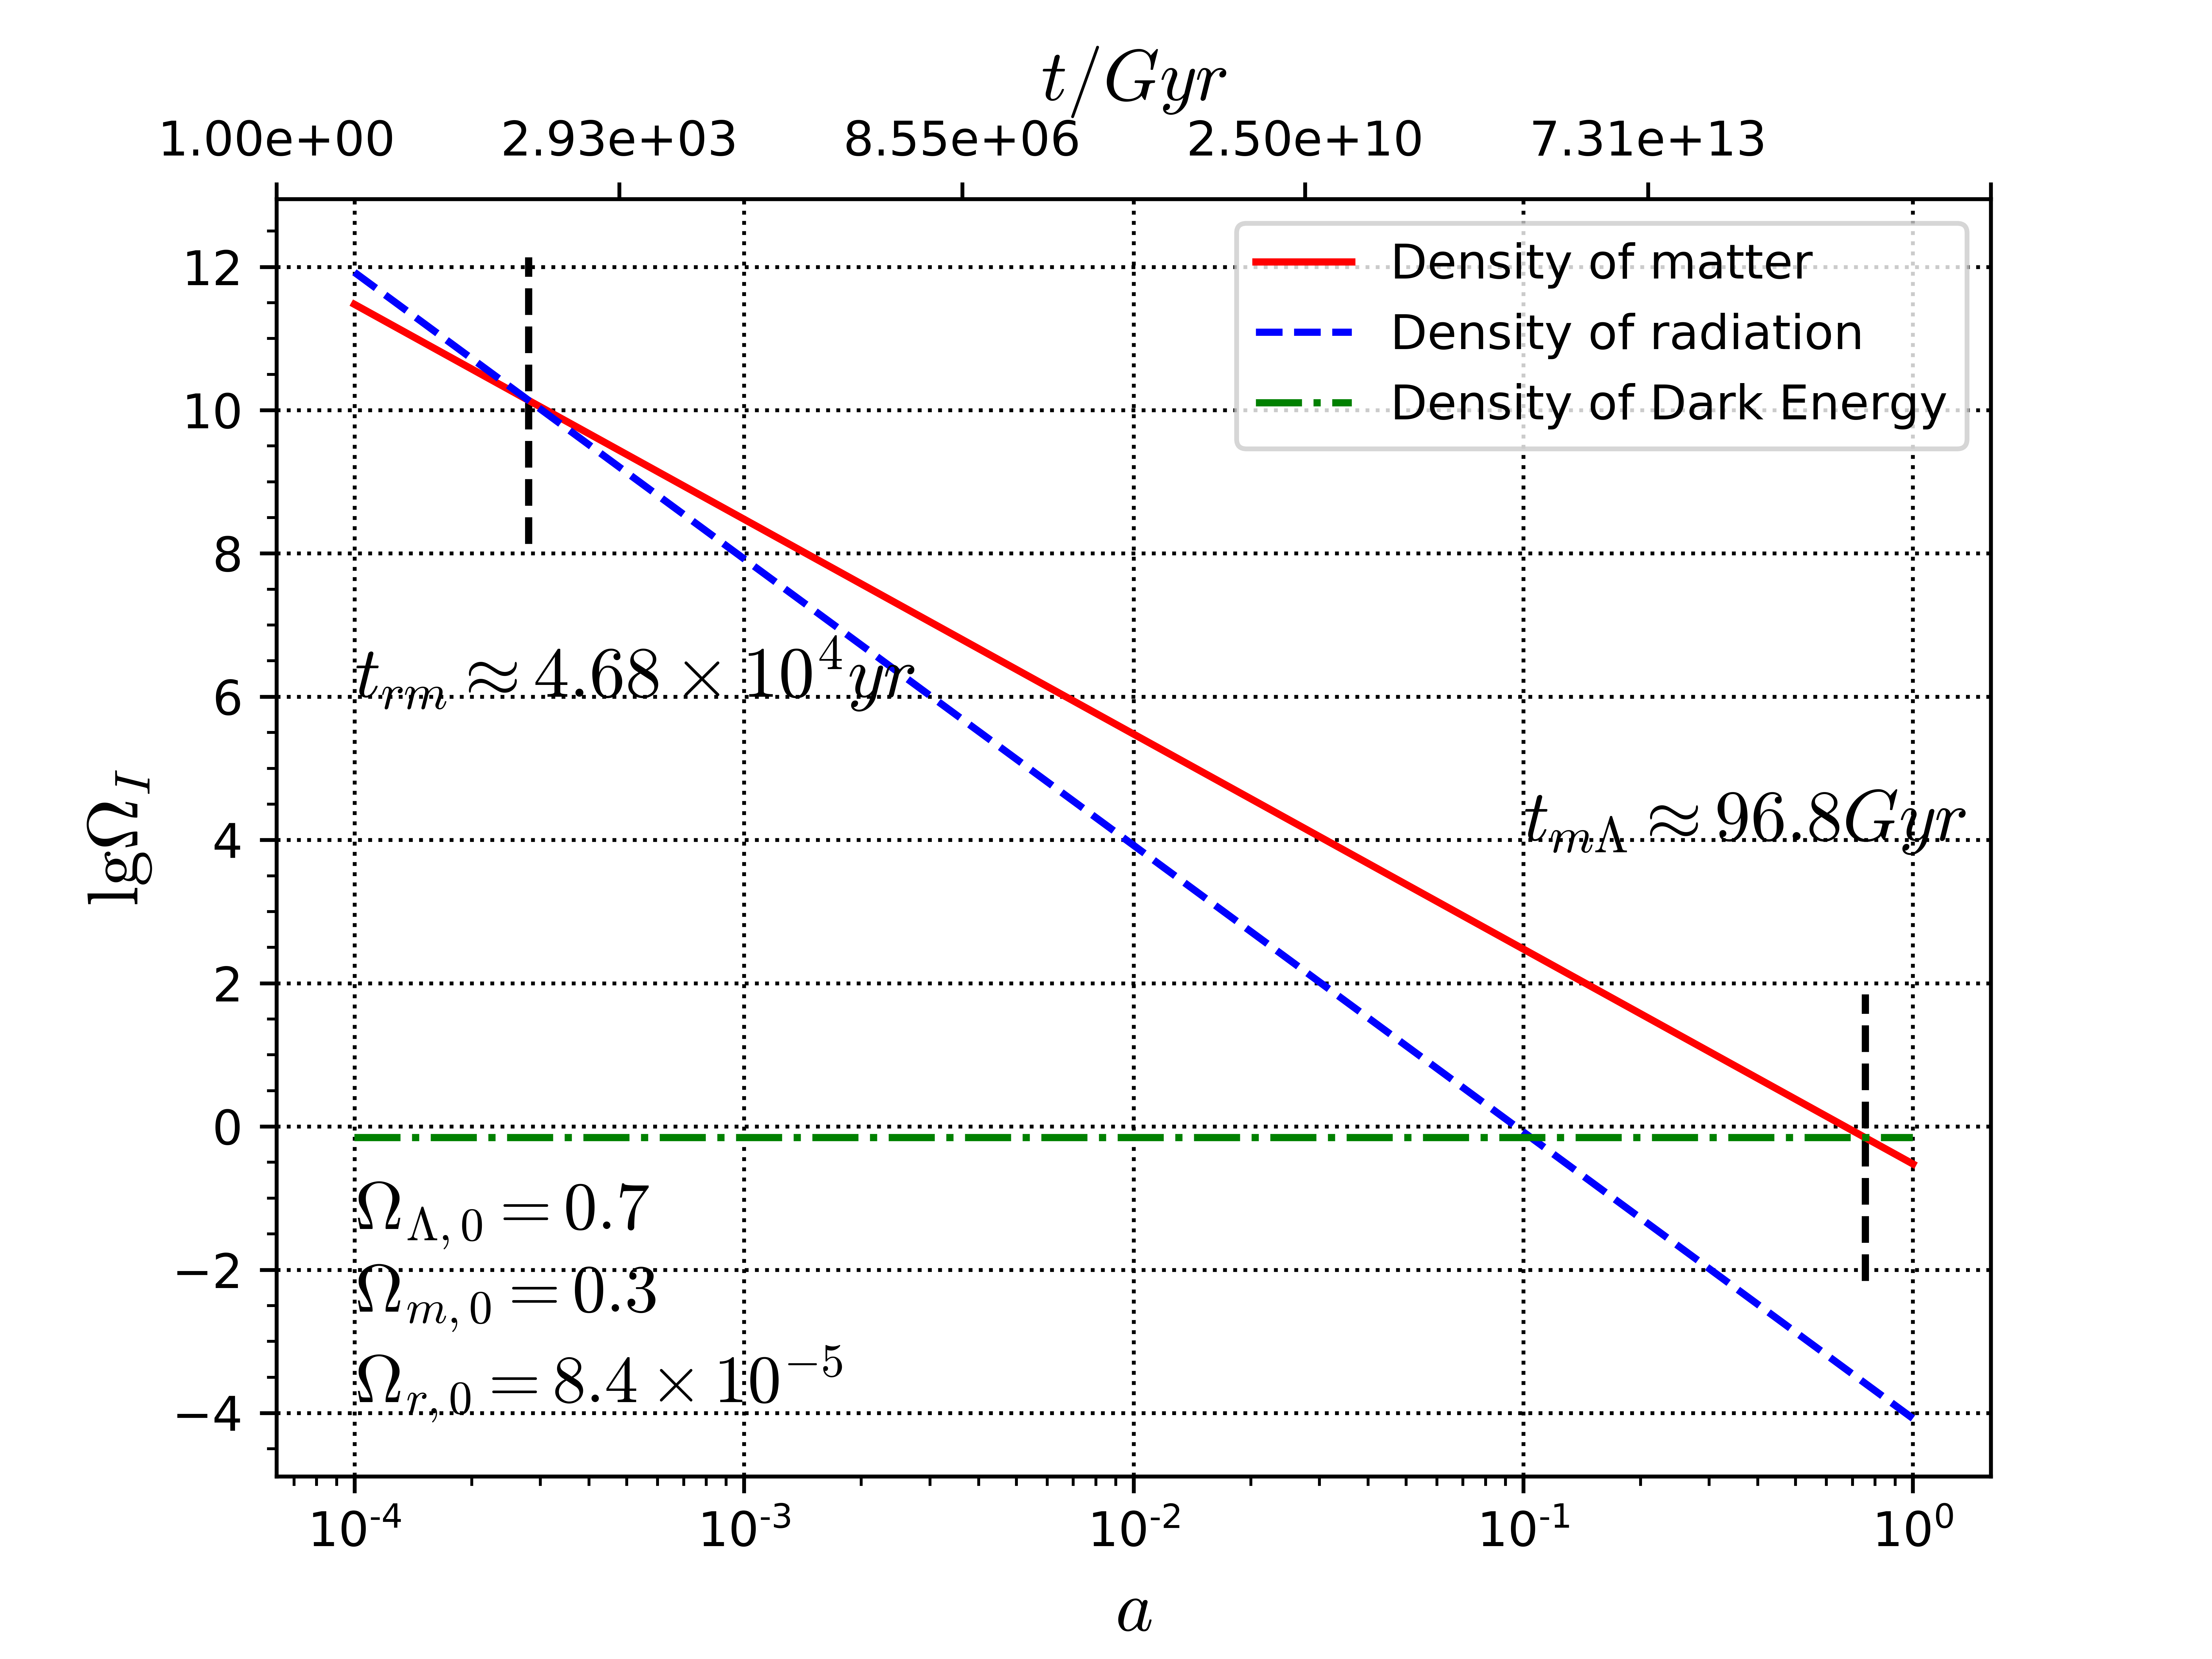
\includegraphics[scale=1]{R2M_Eralog.png}
\caption{\textbf{The evolution of matter density and radiation density over time}}
\end{figure}


\textbf{The moment that universe began to expand in acceleration:}

\begin{align*}
    q_{c}&=\frac{\Omega_{m}}{2}-\Omega_{\Lambda}\\
    &=\frac{\Omega_{m,0}}{2}\frac{a^{-3}_{c}}{a^{-3}_{0}}-\Omega_{\Lambda,0}=0\tag{1.5.6}\\
    a_{c}&=\displaystyle(\frac{\Omega_{m,0}}{2\Omega_{\Lambda}})^{1/3} \approx 0.598 \tag{1.5.7}\\
    z_{c}&=\frac{a_{0}}{a_{c}}-1\approx 0.671 \tag{1.5.8}\\
     t_{c}&=\frac{1}{H_{0}}\int^{\infty}_{z_{c}}\displaystyle\frac{dz}{(1+z)E(z)^{1/2}}\\
      &\approx 96.8 \mathrm{G} yr\tag{1.5.9}
\end{align*}
\subsection{Big Bang Existence Criterion\cite{GRAIfPh1}}
\quad\\
\textbf{Big Bang critical condition:}
\begin{align*}
H^{2}&=H^{2}_{0}[\Omega_{\Lambda,0}+(1-\Omega_{m,0}-\Omega_{\Lambda,0})a^{-2}_{c}+\Omega_{m,0}a^{-3}_{c}]=0\tag{1.6.1}
\end{align*}
\textbf{Which can be re-express as:}
\[
4(1-\Omega_{m,0}-\Omega_{\Lambda,0})+27\Omega_{m,0}^{2}\Omega_{\Lambda,0}=0\tag{1.6.2}
\]
\textbf{By introducing the following variable:}
\[
x=\displaystyle(\frac{\Omega_{\Lambda,0}}{4\Omega_{m,0}})\tag{1.6.3}
\]
\textbf{1.6.2 equation quickly reduces to:}
\[
x^{3}-\frac{3}{4}x-\frac{1-\Omega_{m,0}}{\Omega_{m,0}}=0\tag{1.6.4}
\]
\quad\\
\textbf{Assume that $\Omega_{\Lambda,0}>0$,we can get the following three cases:}

\begin{itemize}
    \item $0<\Omega_{m,0}\le \displaystyle\frac{1}{2}$\\
    \[\Omega_{\Lambda,0}=4\Omega_{m,0}\cosh[\frac{1}{3}\cosh^{-1}(\frac{1-\Omega_{m,0}}{\Omega_{m,0}})]\tag{1.6.5}\]
    \item $\displaystyle\frac{1}{2}<\Omega_{m,0}\le 1$\\
     \[\Omega_{\Lambda,0}=4\Omega_{m,0}\cos[\frac{1}{3}\cos^{-1}(\frac{1-\Omega_{m,0}}{\Omega_{m,0}})]\tag{1.6.6}\]
    \item $\Omega_{m,0}> 1$\\
    \[\Omega_{\Lambda,0}=4\Omega_{m,0}\cos[\frac{1}{3}\cos^{-1}(\frac{1-\Omega_{m,0}}{\Omega_{m,0}})+\frac{4\pi}{3}]\tag{1.6.7}\]
\end{itemize}



\pagebreak
\begin{figure}[H]
\centering
\includegraphics[scale=1]{Universes.png}
\caption{\textbf{FRLW Universe by different cosmological parameters}}
\end{figure}

\pagebreak
\bibliographystyle{plain}
\bibliography{references}
\end{document}